%  Capítulo 2 – Referencial Teórico
% ============================================================

% ============================================================
\section{Previsão de Geração de Energia Fotovoltaica}
\label{sec:previsao_fv}
% ------------------------------------------------------------

\subsection{Especificidades para sistemas fotovoltaicos}
\label{subsec:especificidades_fv}

% TODO: Tratar sazonalidade diária e anual, ausência de geração noturna,
%       impacto de nuvens e aerossóis. Discutir normalização pela irradiância
%       (clear-sky index) como estratégia comum na literatura.

% ============================================================

A série temporal de geração de energia de uma usina fotovoltaica não constitui um sinal
arbitrário: ela resulta da modulação de uma forçante astronômica determinística, a
trajetória solar, por um conjunto de fatores atmosféricos de natureza estocástica. Dessa
dupla origem decorre um conjunto de propriedades estatísticas particulares que distinguem o
problema da previsão fotovoltaica de outras tarefas de previsão de séries temporais e que
condicionam diretamente as escolhas de modelagem, de engenharia de \emph{features} e de
validação adotadas neste trabalho. Esta subseção discute quatro dessas especificidades.

A geração fotovoltaica exibe forte autocorrelação, isto é, dependência estatística entre
valores da série separados por um intervalo de tempo. Em escalas curtas, essa dependência
é elevada e decai monotonicamente com a defasagem, instantes consecutivos apresentam
condições de irradiância e de carga muito semelhantes, de modo que a potência em um dado
instante é fortemente preditiva da potência nos instantes imediatamente seguintes
\cite{Zhou2022}. Essa propriedade é precisamente o que viabiliza as abordagens orientadas
por dados, e fundamenta a construção de preditores baseados em defasagens (\emph{lags}) e em médias móveis da série, que reintroduzem explicitamente essa memória temporal no vetor de entrada dos modelos. Importante salientar, contudo, que a autocorrelação não se restringe a defasagens curtas e dependendo do horizonte escolhido pode ser utilizado defasagens de mais de 24 horas.

A característica mais marcante da série de geração fotovoltaica é a presença de
sazonalidade múltipla, ou seja, a superposição de ciclos periódicos de diferentes
frequências. Dois ciclos predominam. O primeiro é o ciclo diário no qual a geração segue,
a cada dia, um perfil aproximadamente em forma de sino, nulo durante a noite, crescente
após o nascer do Sol, máximo ao redor do meio-dia solar e decrescente até o pôr do Sol. O
segundo é o ciclo anual, a amplitude e a duração desse perfil diário variam ao longo
do ano, em função da declinação solar e dos regimes sazonais de nebulosidade. A
manifestação conjunta dessas periodicidades é diretamente observável na distribuição
temporal do erro dos modelos de previsão, que tende a ser maior nas horas centrais do dia e
nos meses de maior irradiância, justamente onde a magnitude da geração é mais elevada
\cite{Kappler2024}. Essa estrutura sazonal determinística é, em grande medida, conhecida a
priori e pode ser fornecida ao modelo por meio de variáveis astronômicas, como elevação,
azimute e declinação solar, conforme adotado neste trabalho.

A potência gerada é uma grandeza fisicamente não-negativa e limitada superiormente
pela capacidade nominal da usina. Mais relevante do ponto de vista estatístico é o
fenômeno do truncamento diurno, ou seja, durante o período noturno, a geração é
identicamente nula, o que faz com que uma fração substancial das observações da série
assuma exatamente o valor zero, consequentemente, esse efeito distorce a distribuição da variável-alvo, tornando-a fortemente assimétrica e concentrada em zero, a ponto de que a mediana das
observações pode situar-se próxima de zero quando as amostras noturnas são contabilizadas
\cite{Andrade2023}. Tal característica tem duas implicações metodológicas. A primeira diz
respeito ao pré-processamento, no qual parte da literatura opta por remover as observações noturnas do conjunto de dados, tornando a série resultante mais homogênea e estacionária
\cite{Khalyasmaa2020}, enquanto outra parte as preserva, sob o argumento de que o modelo deve operar também nessas condições no cotidiano \cite{Andrade2023}. A segunda implicação refere-se à
própria saída do modelo na qual previsões fisicamente inconsistentes, como valores negativos ou
geração noturna não nula, devem ser tratadas, seja por truncamento explícito a zero, seja
pela imposição de limites dependentes do tempo derivados da geometria solar
\cite{Markovics2022}.

Por fim, a série de geração fotovoltaica é não-estacionária: suas propriedades
estatísticas, como média, variância e estrutura de autocorrelação, não permanecem constantes
ao longo do tempo. Parte dessa não-estacionariedade é determinística e decorre das próprias
sazonalidades já descritas, sendo, portanto, previsível. Outra parte, contudo, é induzida
por fatores externos de evolução lenta ou abrupta, tais como a degradação progressiva dos
módulos, o acúmulo de sujidade (\emph{soiling}) sobre as superfícies, o sombreamento
sazonal por obstáculos, falhas de equipamento e intervenções de manutenção. Esses fatores
alteram a relação entre a forçante meteorológica e a potência efetivamente gerada,
introduzindo mudanças no regime da série que não são explicáveis apenas pelas variáveis de
entrada. Do ponto de vista da modelagem, a não-estacionariedade impõe cautela, uma vez que um modelo ajustado a um período pode degradar seu desempenho quando aplicado a um período posterior
de regime distinto, o que reforça a necessidade de procedimentos de validação que
respeitem a ordem cronológica dos dados — tema retomado na
Subseção~\ref{subsec:cross_validation}.

Em síntese, a previsão de geração fotovoltaica é um problema de série temporal de natureza
particular, no qual uma estrutura determinística forte e conhecível, os ciclos solares,
coexiste com uma componente estocástica e não-estacionária das condições atmosféricas e do
estado das usinas. Dessa maneira, as decisões metodológicas adotadas neste trabalho, da seleção
de variáveis à estratégia de validação, pode ser compreendida como uma resposta direta a
essas quatro especificidades.

\subsection{Diferentes métodos de previsão}
\label{subsec:metodos_previsao}

% TODO: Classificar os métodos existentes: físicos/NWP, estatísticos (ARIMA etc.),
%       baseados em imagens de satélite/céu e baseados em ML/DL.
%       Discutir vantagens e limitações de cada abordagem.
%       Referências-chave: \citep{Antonanzas2016}, \citep{Voyant2017}.

% ------------------------------------------------------------

A literatura especializada propõe diferentes taxonomias para organizar os métodos
de previsão de geração fotovoltaica. Uma classificação recorrente, adotada por
\citeonline{Andrade2023}, distingue quatro classes: métodos físicos, estatísticos, de
inteligência artificial e híbridos. Neste trabalho, contudo, adota-se a partição mais
parcimoniosa proposta por \cite{Markovics2022}, na qual as abordagens de
inteligência artificial são compreendidas como um subconjunto das estatísticas,
resultando em três categorias: físicas, estatísticas e híbridas.
Essa escolha decorre do fato de que tanto os modelos estatísticos clássicos quanto os
de aprendizado de máquina compartilham a característica essencial de serem orientados
por dados (\textit{data-driven}), o que justifica seu agrupamento sob uma mesma categoria
conceitual.

Antes de detalhar cada classe, convém estabelecer a notação comum. Seja $\hat{P}_{ac}(t+h)$
a previsão da potência elétrica em corrente alternada gerada pela usina no instante
$t+h$, em que $t$ é o instante de emissão da previsão e $h$ o horizonte de previsão.
As abordagens distinguem-se, essencialmente, pela forma como modelam o mapeamento entre
as variáveis disponíveis no instante $t$ e essa grandeza-alvo.

Os métodos físicos baseiam-se em cadeias de modelos (\textit{model chains}) que descrevem
analiticamente os processos envolvidos na conversão da energia solar em energia elétrica
\cite{Markovics2022}. A entrada da cadeia é a irradiância prevista por modelos de
Previsão Numérica do Tempo (\textit{Numerical Weather Prediction} --- NWP) ou estimada a
partir de imagens de satélite \cite{Andrade2023}. Por essa razão, a abordagem é também
denominada indireta, pois a potência é obtida pela composição sucessiva de
submodelos, e não diretamente a partir de dados de operação \cite{Markovics2022}.

Formalmente, a cadeia pode ser representada como uma composição de funções
\begin{equation}
    \hat{P}_{ac} = (f_{\mathrm{conv}} \circ f_{\mathrm{trans}} \circ f_{\mathrm{sep}})(G_{h}, \boldsymbol{\theta}),
    \label{eq:model_chain}
\end{equation}
em que $G_{h}$ é a irradiância horizontal global (GHI) prevista e $\boldsymbol{\theta}$
reúne os parâmetros de projeto da usina, como orientação, inclinação, potência nominal e
coeficientes do módulo. Cada operador corresponde a uma etapa física:

\begin{enumerate}
    \item \textbf{Separação das componentes} ($f_{\mathrm{sep}}$): decompõe a GHI em suas
    parcelas direta normal ($G_{b}$) e difusa ($G_{d}$), uma vez que apenas a GHI costuma
    estar disponível. Modelos de separação estimam a fração difusa $k_{d} = G_{d}/G_{h}$
    como função do índice de claridade $k_{t} = G_{h}/G_{0}$, sendo $G_{0}$ a irradiância
    extraterrestre no plano horizontal \cite{Markovics2022}.

    \item \textbf{Transposição para o plano inclinado} ($f_{\mathrm{trans}}$): converte as
    componentes no plano horizontal para a irradiância no plano dos módulos ($G_{t}$),
    geralmente segundo
    \begin{equation}
        G_{t} = G_{b}\cos\theta_{i} + G_{d}\,R_{d} + \rho\,G_{h}\,R_{r},
        \label{eq:transposicao}
    \end{equation}
    em que $\theta_{i}$ é o ângulo de incidência, $R_{d}$ e $R_{r}$ são os fatores de
    transposição das componentes difusa e refletida, e $\rho$ é o albedo do solo.

    \item \textbf{Conversão irradiância-potência} ($f_{\mathrm{conv}}$): modela a eficiência
    do sistema, incorporando o efeito da temperatura de operação. Uma forma usual é
    \begin{equation}
        P_{ac} = \eta_{\mathrm{inv}}\,P_{\mathrm{nom}}\,\frac{G_{t}}{G_{\mathrm{STC}}}
        \left[1 + \gamma\,(T_{mod} - T_{\mathrm{STC}})\right],
        \label{eq:conversao}
    \end{equation}
    em que $P_{\mathrm{nom}}$ é a potência nominal, $G_{\mathrm{STC}} = 1000~\mathrm{W/m^2}$
    e $T_{\mathrm{STC}} = 25~^{\circ}\mathrm{C}$ são as condições-padrão de ensaio (STC),
    $\gamma < 0$ é o coeficiente de temperatura de potência, $\eta_{\mathrm{inv}}$ a
    eficiência do inversor, e a temperatura do módulo $T_{mod}$ é estimada a partir de
    $T_{amb}$, $G_{t}$ e da velocidade do vento por correlações empíricas, e.g.,
    $T_{mod} = T_{amb} + (G_{t}/G_{\mathrm{ref}})\,(T_{\mathrm{NOCT}} - 20)$
    \cite{Sohani2022}.
\end{enumerate}

Em aplicações de maior fidelidade, $f_{\mathrm{conv}}$ pode substituir a
Equação~\eqref{eq:conversao} por um modelo eletricamente fundamentado do módulo, como o
modelo de diodo único, cuja relação corrente-tensão é dada por
\begin{equation}
    I = I_{ph} - I_{0}\left[\exp\!\left(\frac{V + I R_{s}}{n V_{t}}\right) - 1\right]
    - \frac{V + I R_{s}}{R_{p}},
    \label{eq:diodo}
\end{equation}
em que $I_{ph}$ é a fotocorrente (proporcional a $G_{t}$), $I_{0}$ a corrente de saturação,
$V_{t}$ a tensão térmica, $n$ o fator de idealidade, e $R_{s}$, $R_{p}$ as resistências
série e paralela \cite{Sohani2022}.

A principal vantagem dessa abordagem é não exigir dados históricos de operação, já que
descreve o comportamento da usina a partir de seus parâmetros de projeto, os modelos
físicos, portanto, podem ser implementados antes mesmo de a usina entrar em operação
\cite{Andrade2023}. Em contrapartida, apresentam, em geral, acurácia inferior à dos métodos
orientados por dados e demandam conhecimento detalhado das especificações da planta
\cite{Markovics2022,Andrade2023}. Adicionalmente, a seleção dos submodelos que compõem cada
elo da cadeia (separação, transposição e conversão) exerce impacto considerável sobre a
acurácia final \cite{Markovics2022}, e os erros de cada etapa propagam-se ao longo da
composição da Equação~\eqref{eq:model_chain}.

Já os métodos estatísticos abrangem toda a gama de abordagens orientadas por dados, desde os
modelos estatísticos clássicos até as técnicas de aprendizado de máquina
\cite{Markovics2022}. O traço comum é estimar, a partir de um conjunto de dados históricos
$\{(\mathbf{x}_{i}, y_{i})\}_{i=1}^{N}$, uma função $\hat{f}$ que minimize uma função de
perda $\mathcal{L}$ sobre esses dados,
\begin{equation}
    \hat{f} = \arg\min_{f \in \mathcal{F}} \frac{1}{N}\sum_{i=1}^{N}
    \mathcal{L}\big(y_{i}, f(\mathbf{x}_{i})\big),
    \label{eq:erm}
\end{equation}
sendo $\mathcal{F}$ a classe de funções admissíveis e, tipicamente, $\mathcal{L}$ o erro
quadrático $\mathcal{L}(y,\hat{y}) = (y-\hat{y})^{2}$. A potência prevista é então
$\hat{P}_{ac}(t+h) = \hat{f}(\mathbf{x}_{t})$.

Os modelos diferenciam-se pela natureza do vetor de entrada $\mathbf{x}_{t}$ e pela classe
$\mathcal{F}$. Nos modelos autorregressivos clássicos, como os da família ARIMA, a
entrada é constituída pelos próprios valores passados da série de geração e dos erros
passados. Um modelo ARMA($p,q$), por exemplo, assume
\begin{equation}
    y_{t} = c + \sum_{i=1}^{p}\phi_{i}\,y_{t-i}
    + \sum_{j=1}^{q}\vartheta_{j}\,\varepsilon_{t-j} + \varepsilon_{t},
    \label{eq:arma}
\end{equation}
em que $\phi_{i}$ e $\vartheta_{j}$ são, respectivamente, os coeficientes autorregressivos
e de média móvel, e $\varepsilon_{t}$ é um ruído branco \cite{Andrade2023}. Dessa forma, esses modelos
são capazes de capturar dependências lineares na estrutura temporal da série, mas têm capacidade limitada
de representar as relações fortemente não lineares entre as variáveis meteorológicas e a
potência gerada.

Já os modelos de aprendizado de máquina (\textit{machine learning}) ampliam a classe $\mathcal{F}$ para famílias
não lineares e admitem como entrada um vetor de variáveis exógenas $\mathbf{x}_{t}$, como
irradiância, temperatura ambiente, velocidade do vento e ângulos solares.
Exemplos comuns na literatura de previsão fotovoltaica incluem máquinas de vetores de
suporte (\emph{Support Vector Machines}, SVM), florestas aleatórias (\emph{Random Forests}) e
redes neurais artificiais \cite{Andrade2023}. 

A principal vantagem operacional dos métodos estatísticos reside em não requererem
conhecimento dos parâmetros de projeto da usina, o que facilita sua implementação
\cite{Markovics2022}, sendo, dessa maneira, um atributo particularmente relevante para operadores que não dispõem
das especificações de parques distribuídos. Entre eles, as técnicas de aprendizado de
máquina são as mais empregadas \cite{Markovics2022} e, embora frequentemente apresentem os
melhores resultados, costumam exigir maior esforço computacional \cite{Andrade2023}. Como
limitações, herdam a dependência da quantidade e da qualidade dos dados de treinamento e
estão sujeitas a sobreajuste (\emph{overfitting}) quando a complexidade de $\mathcal{F}$
não é adequadamente regularizada.

Por último, os métodos híbridos combinam elementos físicos e estatísticos em diferentes configurações,
constituindo uma categoria abrangente que se refere à hibridização de quaisquer duas ou
mais abordagens das classes anteriores \cite{Markovics2022,Andrade2023}. Um exemplo
representativo é o pré-processamento físico da irradiância prevista por modelos NWP como
variável de entrada para um modelo de aprendizado de máquina. Nesse arranjo, a etapa física
fornece uma estimativa fisicamente consistente da irradiância no plano dos módulos, $G_{t}$,
e o modelo estatístico assume a conversão irradiância-potência, isto é,
\begin{equation}
    \hat{P}_{ac}(t+h) = \hat{f}\big(f_{\mathrm{trans}}(f_{\mathrm{sep}}(G_{h})),
    T_{amb}, V_{w}, \dots\big),
    \label{eq:hibrido}
\end{equation}
substituindo a conversão analítica das Equações~\eqref{eq:conversao}--\eqref{eq:diodo} por
um mapeamento aprendido dos dados.

Nesse cenário, a motivação é explorar a complementaridade entre as abordagens. \citeonline{Markovics2022}
verificam que a incorporação, ao conjunto de preditores de um modelo de aprendizado de
máquina, de variáveis calculadas analiticamente, como os ângulos de posição do Sol
(elevação, azimute e declinação), aprimoram de forma significativa a acurácia das previsões
de potência. Esse resultado evidencia que a fronteira entre as categorias é, na prática,
permeável, e sugere que a engenharia de \emph{features} de base física constitui uma forma
de hibridização de baixo custo e elevado retorno.

\subsection{Horizontes temporais de previsão}
\label{subsec:horizontes_temporais}

% TODO: Definir os horizontes: very short-term (< 1 h), short-term (1–48 h),
%       medium-term (dias) e long-term (semanas/meses).
%       Relacionar cada horizonte com as necessidades do operador de rede.

% ------------------------------------------------------------

A previsão de geração fotovoltaica não constitui um problema único, mas uma família de
problemas cujas variáveis de entrada relevantes, técnicas adequadas e
aplicações de destino variam acentuadamente conforme o horizonte de previsão
considerado, isto é, o intervalo de tempo entre o instante de emissão da previsão e o
instante previsto. Conforme observam \citeonline{Tian2023}, os valores de irradiância e
de potência mantêm forte relação com a escala temporal, de modo que a definição do
horizonte condiciona toda a estratégia de modelagem. A partir desse contexto, esta subseção apresenta, de forma
comparativa, as principais faixas de horizonte usualmente distinguidas na literatura,
situando ao final a opção adotada neste trabalho.

Com efeito, embora não exista uma fronteira universalmente padronizada entre as faixas, a literatura
converge para uma divisão em quatro classes, sendo elas a previsão de altíssimo curto prazo
(\emph{nowcasting} ou intra-hora), a de curto prazo (intra-dia), a de um dia à frente
(\emph{day-ahead}) e a de médio a longo prazo. O traço que melhor as distingue não é apenas
a duração, mas a natureza física dominante da incerteza em cada escala e, por
consequência, a fonte de informação mais adequada para reduzi-la.

\subsubsection*{Altíssimo curto prazo (nowcasting)}

Nessa faixa, que abrange de segundos a aproximadamente uma hora à frente, a variabilidade
da geração é governada quase exclusivamente pelo movimento de nuvens, que provoca rampas
abruptas de irradiância em escala de segundos a minutos. Dessa maneira, as técnicas mais eficazes são as
que capturam o estado instantâneo do céu, como imageadores de céu total (\emph{sky imagers}),
que extraem vetores de movimento de nuvens (\emph{cloud motion vectors}) a partir de
imagens hemisféricas, e modelos puramente autorregressivos baseados em medições de alta
frequência da própria usina \cite{Tian2023}. Além disso, modelos de Previsão Numérica do Tempo (NWP),
são inadequados nessa escala por sua resolução temporal e latência de processamento. As
aplicações típicas incluem o controle em tempo real de inversores, a gestão de rampas e a
operação coordenada com sistemas de armazenamento por baterias.

\subsubsection*{Curto prazo (intra-dia)}

Estendendo-se de aproximadamente uma hora a seis horas à frente, essa faixa caracteriza-se, especialmente,
pela transição entre o regime dominado por nuvens e aquele dominado pela dinâmica
atmosférica de meso-escala. As abordagens mais empregadas combinam a extrapolação de
imagens de satélite que oferecem cobertura espacial superior à dos imageadores de solo
com modelos estatísticos e de aprendizado de máquina alimentados por séries temporais
recentes \cite{Tian2023}. As aplicações estão associadas ao despacho intra-dia, ao
mercado de curto prazo e ao balanceamento operacional do sistema.

\subsubsection*{Um dia à frente (day-ahead)}

A previsão \emph{day-ahead}, comumente entendida como o horizonte de 24 a 48 horas à
frente, é a de maior relevância para a operação e a comercialização de energia, pois é a
escala em que tipicamente se programa o despacho do dia seguinte e se submetem as ofertas
ao mercado \cite{Markovics2022}. Nessa faixa, o movimento individual de nuvens já não é
previsível de forma determinística, o que conduz a duas estratégias distintas quanto à
informação utilizada. A primeira recorre à Previsão Numérica do Tempo (NWP), cujas
previsões de irradiância e demais variáveis meteorológicas para o dia seguinte alimentam
modelos de conversão irradiância-potência \cite{Markovics2022}. A segunda, de natureza
puramente endógena, dispensa qualquer informação meteorológica futura e projeta a geração
do dia seguinte exclusivamente a partir do histórico de geração e das variáveis medidas na
própria usina até o instante de emissão da previsão, explorando a estrutura de
autocorrelação e os padrões diários e sazonais da série temporal. Diversos estudos da
literatura adotam essa segunda estratégia, utilizando como preditores a potência gerada e
as variáveis meteorológicas observadas em períodos anteriores \cite{Andrade2023}.

A abordagem endógena apresenta a vantagem prática de não requerer acesso a previsões NWP ao custo de uma acurácia tipicamente inferior à da abordagem
baseada em NWP, uma vez que se abstém da principal fonte de informação sobre as condições
atmosféricas futuras. Trata-se, portanto, de um compromisso entre disponibilidade de dados
e desempenho preditivo.

\subsubsection*{Médio e longo prazo}

Para horizontes que vão de alguns dias a meses ou anos, a previsibilidade da geração em um
instante específico essencialmente se perde, e o objeto da previsão desloca-se de valores
instantâneos para grandezas agregadas como médias diárias, mensais, sazonais ou anuais
\cite{Tian2023}. Predomina aqui a chamada previsão generalizada, na qual cada
conjunto de entradas corresponde a um valor agregado de saída \cite{Tian2023}. As
aplicações típicas situam-se no planejamento energético, no dimensionamento de ativos e na
estimativa de produção de longo prazo para fins de análise de viabilidade.

\subsubsection*{Síntese comparativa}

A Tabela~\ref{tab:horizontes} sintetiza as quatro faixas discutidas, contrastando o
horizonte, a fonte física dominante da variabilidade, as técnicas predominantes e as
principais aplicações.

\begin{table}[htb]
    \centering
    \caption{Comparativo das faixas de horizonte temporal de previsão de geração fotovoltaica.}
    \label{tab:horizontes}
    \begin{tabular}{p{2.4cm} p{2.0cm} p{3.4cm} p{3.2cm}}
        \toprule
        \textbf{Faixa} & \textbf{Horizonte típico} & \textbf{Técnicas predominantes} & \textbf{Aplicações principais} \\
        \midrule
        Altíssimo curto prazo (\emph{nowcasting}) & Segundos a $\sim$1\,h &
        Imageadores de céu total, vetores de movimento de nuvens, modelos autorregressivos &
        Controle de inversores, gestão de rampas, operação de baterias \\
        \addlinespace
        Curto prazo (intra-dia) & $\sim$1\,h a 6\,h &
        Extrapolação de imagens de satélite, aprendizado de máquina &
        Despacho intra-dia, mercado de curto prazo, balanceamento \\
        \addlinespace
        Um dia à frente (\emph{day-ahead}) & 24\,h a 48\,h &
        NWP acoplado a modelos de aprendizado de máquina, ou modelos puramente endógenos sobre séries históricas &
        Programação do despacho, comercialização no mercado diário \\
        \addlinespace
        Médio e longo prazo & Dias a anos &
        NWP de longo alcance, modelos climatológicos, previsão generalizada &
        Planejamento energético, dimensionamento de ativos, análise de viabilidade \\
        \bottomrule
    \end{tabular}
    \begin{flushleft}
    \footnotesize Fonte: elaborado pelo autor a partir de \citeonline{Markovics2022} e \citeonline{Tian2023}.
    \end{flushleft}
\end{table}

A delimitação dessas faixas permite situar com precisão o escopo deste trabalho, que se
concentra no horizonte de \emph{um dia à frente} (\emph{day-ahead}) sob uma abordagem
estritamente endógena, isto é, baseada apenas no histórico das usinas, sem o emprego de
previsões NWP.

Essa escolha justifica-se por dois motivos convergentes. Em primeiro lugar, o horizonte
\emph{day-ahead} é a escala de maior valor operacional e comercial, por coincidir com o
horizonte de programação do despacho e de submissão de ofertas ao mercado, conforme
discutido na Subseção~\ref{subsec:relevancia}. Em segundo lugar, a restrição a dados
endógenos reflete uma condição realista de disponibilidade de dados no contexto brasileiro,
no qual o acesso a previsões NWP de qualidade nem sempre está garantido, e permite avaliar
em que medida a informação contida na própria série histórica das usinas é suficiente para
uma previsão de utilidade operacional. Reconhece-se, contudo, que essa restrição estabelece
um limite superior de acurácia inferior ao alcançável com a incorporação de previsões
meteorológicas futuras, sendo, portanto, uma limitação assumida deliberadamente e discutida adiante na análise
de resultados.

\subsection{Modelos de referência (\textit{baselines})}
\label{subsec:modelos_referencia}

% TODO: Descrever os benchmarks utilizados (e.g., persistência, média histórica,
%       modelo climatológico). Fundamentar a importância de comparar com baselines.

% ------------------------------------------------------------

A avaliação de um modelo de previsão não se esgota na aferição de métricas como o erro quadrático médio (RMSE) ou o erro absoluto médio (MAE), discutidas na
Seção~\ref{sec:metricas}, são fortemente dependentes das características do local, do
horizonte e da resolução temporal dos dados, o que inviabiliza a comparação direta de
resultados obtidos em conjuntos de dados distintos \cite{Markovics2022}. Um RMSE de
determinado valor pode representar um desempenho excelente em um sítio de elevada
variabilidade e medíocre em um sítio de céu estável. Por essa razão, a literatura de
previsão solar recomenda contextualizar o desempenho de qualquer modelo por comparação com
um modelo de referência (\emph{baseline}), isto é, um método simples, de baixo custo, que
estabelece o patamar mínimo de acurácia que um modelo sofisticado deve superar para
justificar sua complexidade \cite{Sarmas2022}.

Essa comparação é formalizada pelo \emph{índice de habilidade preditiva} (\emph{forecast
skill score}), definido como
\begin{equation}
    \mathrm{skill} = 1 - \frac{\mathrm{RMSE}_{\mathrm{modelo}}}{\mathrm{RMSE}_{\mathrm{ref}}},
    \label{eq:skill}
\end{equation}
em que $\mathrm{RMSE}_{\mathrm{modelo}}$ é o erro do modelo proposto e
$\mathrm{RMSE}_{\mathrm{ref}}$ o do modelo de referência \cite{Sarmas2022}. Um valor positivo
indica que o modelo proposto supera o \emph{baseline}, enquanto, um valor nulo, desempenho
equivalente, e um valor negativo, inferior ao da referência. O \emph{skill
score} permite, assim, uma leitura padronizada e adimensional do ganho efetivo do modelo,
ainda que se deva ressalvar que sua comparabilidade entre estudos distintos depende da
adoção de uma mesma referência \cite{Markovics2022}. A seguir, apresentam-se os modelos de
referência usualmente empregados na previsão de geração fotovoltaica.

Primeiro, tem-se o modelo de persistência ingênua (\emph{naïve persistence}) é o mais elementar dos \emph{baselines}. Assume que o valor futuro da grandeza é igual ao seu último valor
observado,
\begin{equation}
    \hat{y}(t + \Delta t) = y(t),
    \label{eq:persistencia_naive}
\end{equation}
em que $\Delta t$ é o horizonte de previsão. Embora seja um referencial trivial e de
desempenho razoável em horizontes muito curtos, a persistência ingênua é manifestamente
inadequada para a geração fotovoltaica em horizontes de horas ou mais, pois ignora por
completo o ciclo diário da irradiância, ou seja, prevê que a geração das 18\,h será igual à do meio-dia, produzindo, assim, erros grosseiros. Por isso, sua utilização isolada como referência é desencorajada na literatura de previsão solar, que a
considera um patamar excessivamente baixo, capaz de superestimar artificialmente a
habilidade do modelo avaliado \cite{Sarmas2022}.

Para contornar essa limitação, a literatura recomenda o uso da persistência
inteligente (\emph{smart persistence}) como referência \cite{Sarmas2022}, em que a ideia central é separar a componente determinística da geração, o ciclo solar, de sua
componente estocástica, isto é, as flutuações associadas às condições atmosféricas. Define-se,
primeiro, um modelo de céu claro (\emph{clear-sky model}), que fornece a potência
esperada $y_{cs}(t)$ que a usina geraria sob condições de céu limpo em cada instante,
função determinística da hora do dia e do dia do ano. A persistência inteligente assume,
então, que a razão entre a geração observada e a geração de céu claro, o chamado
índice de céu claro, permanece constante ao longo do horizonte:
\begin{equation}
    \hat{y}(t + \Delta t) =
    \begin{cases}
        y_{cs}(t + \Delta t), & \text{se } y_{cs}(t) = 0, \\[6pt]
        y_{cs}(t + \Delta t)\,\dfrac{y(t)}{y_{cs}(t)}, & \text{caso contrário,}
    \end{cases}
    \label{eq:smart_persistence}
\end{equation}
de modo que, em condições noturnas (quando $y_{cs}(t) = 0$), a previsão iguala-se à própria
potência de céu claro \cite{Sarmas2022}. Essa formulação incorpora ao \emph{baseline} a
estrutura determinística do ciclo solar, elevando-o a um patamar de comparação muito mais
exigente e fisicamente coerente. A persistência inteligente é, por isso, o modelo de
referência recomendado e mais amplamente adotado na previsão de geração fotovoltaica
\cite{Sarmas2022, Markovics2022}. Cabe notar que o modelo de céu claro pode ser construído de
forma empírica, por exemplo pela média dos valores históricos de potência condicionada à
hora do dia e ao dia do ano \cite{Sarmas2022}.

Além desses dois, há um terceiro grupo de referências, de complexidade intermediária, é composto por modelos estatísticos clássicos, como a regressão linear e os modelos autorregressivos da família ARIMA, já descritos na Subseção~\ref{subsec:metodos_previsao}. No entanto, diferentemente da persistência, esses modelos são efetivamente ajustados aos dados, capturando dependências lineares na série e entre as variáveis. Seu papel como \emph{baseline} é distinto do da persistência, pois enquanto esta estabelece o piso mínimo a ser superado, um modelo linear estabelece um referencial mais informativo, que isola especificamente o ganho atribuível à capacidade de modelar relações não lineares. Se um modelo de aprendizado de máquina
não supera, ou supera apenas marginalmente, uma regressão linear sobre o mesmo conjunto de
variáveis, há indício de que a complexidade adicional não se justifica para o problema em
questão \cite{Markovics2022}.


A definição do conjunto de modelos de referência a ser efetivamente adotado neste trabalho
é apresentada no Capítulo~\ref{cap:materiais_metodos}. De modo geral, a literatura sugere o
emprego conjunto de \emph{baselines} de diferentes níveis de sofisticação com a persistência
inteligente como referência canônica que ancora o cálculo do \emph{skill score} e
assegura a comparabilidade com outros estudos da área e ao menos um modelo estatístico
linear, que permite quantificar o ganho marginal proporcionado pela modelagem não linear.
Essa estratificação dos referenciais confere robustez à avaliação, ao distinguir entre o
ganho sobre um patamar trivial e o ganho sobre uma alternativa já não trivial.

\subsection{Abordagem utilizada}
\label{subsec:abordagem_utilizada}

% TODO: Justificar a escolha do horizonte e da abordagem de ML adotada.
%       Descrever se a previsão é day-ahead, intraday etc.
%       Explicar o pipeline geral: entrada → modelo → saída.

% ------------------------------------------------------------
\section{Aprendizado de Máquina para Séries Temporais}
\label{sec:ml_series_temporais}

% ------------------------------------------------------------
\subsection{Fundamentos do aprendizado de máquina}
\label{subsec:fundamentos_ml}

O aprendizado de máquina pode ser entendido como o conjunto de técnicas que
permitem a um algoritmo melhorar seu desempenho em uma tarefa a partir da
experiência adquirida com dados, sem que as regras de mapeamento sejam
explicitamente programadas \cite{hastie2009}. A partir disso, no contexto deste trabalho, a
tarefa é de aprendizado supervisionado, modalidade na qual o algoritmo dispõe,
durante o treinamento, de pares de entrada e saída $\{(x_i, y_i)\}_{i=1}^{N}$ e
busca inferir a função subjacente que associa o vetor de preditores $x_i$ ao
valor-alvo $y_i$. Quando o alvo é uma grandeza contínua, por exemplo a potência
ativa gerada pela usina, o problema configura-se como uma regressão, em
oposição às tarefas de classificação, nas quais a saída é categórica
\cite{bishop2006}. A particularidade do problema aqui tratado é que as
observações constituem uma série temporal, isto é, uma sequência de medições
indexadas no tempo e, em geral, mutuamente dependentes, o que impõe
considerações específicas tanto na formulação quanto na avaliação dos modelos.

Conforme já formalizado na Equação~\eqref{eq:erm}, o ajuste de um
modelo consiste em selecionar, dentro de uma classe de funções admissíveis
$\mathcal{F}$, a função $\hat{f}$ que minimiza uma função de perda
$\mathcal{L}$ sobre o conjunto de treinamento. O objetivo último do aprendizado,
contudo, não é minimizar o erro sobre os dados já observados, mas sobre dados
ainda não vistos. Formalmente, deseja-se minimizar o risco esperado, isto é, o
valor esperado da perda sobre a distribuição conjunta $P(x,y)$ que governa o
fenômeno,
%
\begin{equation}
    R(f) = \mathbb{E}_{(x,y)\sim P}\!\left[\mathcal{L}\big(y, f(x)\big)\right],
    \label{eq:risco_esperado}
\end{equation}
%
quantidade que não é diretamente acessível, dado que $P(x,y)$ é desconhecida. Na
prática, minimiza-se o risco empírico, calculado sobre a amostra finita de
treinamento, sob a hipótese de que este aproxima o risco esperado
\cite{vapnik1999}. A discrepância entre ambos caracteriza a capacidade de
generalização de um modelo, propriedade que distingue um sistema que
efetivamente aprendeu padrões transferíveis de um que apenas memorizou as
particularidades da amostra.

Nesse sentido, no caso das séries temporais, a validade dessa aproximação repousa sobre
hipóteses que merecem atenção. Primeiramente, a formulação clássica do risco empírico pressupõe
que as observações sejam independentes e identicamente distribuídas (\textit{i.i.d.}),
suposição evidentemente falsa em dados de geração fotovoltaica, uma vez que as medições
consecutivas exibem forte autocorrelação, ou seja, a potência gerada em um instante
guarda relação direta com a dos instantes vizinhos, além disso, a distribuição
geradora dos dados não é, em rigor, estacionária, pois varia com os ciclos
diário e sazonal e com a degradação dos equipamentos ao longo do tempo
\cite{hyndman2021}. Disso decorre que o desempenho aferido em dados passados só
se transfere ao futuro na medida em que a estrutura estatística da série se
mantenha aproximadamente estável, ressalva que delimita o alcance de qualquer
previsão e que justifica a reavaliação periódica dos modelos em operação.

A formulação supervisionada de uma série temporal é tipicamente obtida pela
construção de uma janela deslizante (\textit{sliding window}), na qual o vetor
de preditores $x_t$ é composto por valores defasados da própria série e por
covariáveis exógenas disponíveis até o instante $t$, enquanto o alvo é o valor
da série no horizonte de previsão $t+h$. Esse procedimento converte a sequência
temporal em um conjunto de pares entrada-saída compatível com a
Equação~\eqref{eq:perda_empirica}, mas introduz uma exigência crítica que nenhuma
informação posterior ao instante de previsão pode integrar o vetor de
preditores, sob pena de vazamento de informação (\textit{data leakage}), que é o uso indevido de dados do futuro durante o treinamento, produzindo, assim,
estimativas de desempenho otimistas e irrealizáveis em operação
\cite{hastie2009}.

Essas considerações conectam-se ao compromisso entre viés e variância
(\textit{bias--variance tradeoff}), que organiza grande parte das decisões de
modelagem. Modelos com capacidade representacional insuficiente, isto é, classe
$\mathcal{F}$ excessivamente restrita, tendem a um erro sistemático elevado,
ou alto viés, falhando em capturar a estrutura dos dados, fenômeno designado por
subajuste (\textit{underfitting}). Inversamente, modelos de capacidade excessiva
ajustam-se ao ruído do conjunto de treinamento, exibindo alta
variância e desempenho deficiente em dados novos, o já mencionado sobreajuste
(\textit{overfitting}) \cite{hastie2009}. Dessa maneira, o erro esperado de generalização pode
ser decomposto na soma de uma componente de viés ao quadrado, uma componente de
variância e um termo de erro irredutível, associado ao ruído intrínseco do
processo, este último inevitável e independente do modelo adotado
\cite{geman1992}. No contexto deste trabalho, esse ruído incorpora a parcela
genuinamente estocástica do fenômeno meteorológico subjacente, o que estabelece
um piso de erro abaixo do qual nenhum modelo pode operar.

O controle desse compromisso é exercido, em larga medida, por meio da
regularização que é um conjunto de técnicas que penalizam a complexidade do
modelo a fim de restringir efetivamente a classe $\mathcal{F}$ e favorecer
soluções mais simples e generalizáveis. Formalmente, para um modelo
parametrizado por um vetor $\boldsymbol{\theta}$, o problema de minimização do
risco empírico enunciado na Equação~\eqref{eq:erm} é substituído por uma versão
penalizada, em que se acresce à função de perda um termo $\Omega(\boldsymbol{\theta})$
que cresce com a complexidade do modelo,
%
\begin{equation}
    \hat{\boldsymbol{\theta}}
    = \arg\min_{\boldsymbol{\theta}}
    \left[
        \frac{1}{N}\sum_{i=1}^{N}
        \mathcal{L}\big(y_i,\, f(x_i;\boldsymbol{\theta})\big)
        + \lambda\,\Omega(\boldsymbol{\theta})
    \right],
    \label{eq:risco_regularizado}
\end{equation}
%
em que $\lambda \geq 0$ é um hiperparâmetro que pondera o compromisso entre a
fidelidade aos dados de treinamento, favorecida pelo primeiro termo, e a
simplicidade do modelo, favorecida pelo segundo. O limite $\lambda \to 0$
recupera a minimização do risco empírico sem penalização, ficando, assim, propensa ao
sobreajuste, ao passo que valores elevados de $\lambda$ restringem mais
severamente a classe efetiva de funções, deslocando o modelo na direção de maior
viés e menor variância. A regularização constitui, dessa maneira, o mecanismo explícito
pelo qual o compromisso viés-variância é operacionalizado durante o ajuste.
As escolhas mais usuais para o termo de penalidade incidem sobre a norma do
vetor de parâmetros. A penalidade $\ell_2$ (\textit{ridge}),
$\Omega(\boldsymbol{\theta}) = \lVert \boldsymbol{\theta} \rVert_2^2
= \sum_{j} \theta_j^2$, encolhe os coeficientes de forma contínua em direção a
zero, sem necessariamente anulá-los, mitigando a sensibilidade do modelo a
variáveis correlacionadas. Já a penalidade $\ell_1$ (\textit{lasso}),
$\Omega(\boldsymbol{\theta}) = \lVert \boldsymbol{\theta} \rVert_1
= \sum_{j} \lvert \theta_j \rvert$, tende a produzir soluções esparsas, anulando
inteiramente os coeficientes de preditores pouco informativos e operando, por
conseguinte, uma forma implícita de seleção de variáveis \cite{hastie2009}.
Além dessas penalidades aplicadas diretamente à função de perda, há mecanismos
de regularização específicos de cada família de modelos, tais como a limitação
da profundidade em árvores de decisão ou a interrupção antecipada
(\textit{early stopping}) no treinamento de redes neurais.

Em síntese, a busca por generalização para além do conjunto de treinamento, o compromisso entre viés e variância e o controle da complexidade por regularização convergem para uma mesma exigência prática de estimar de forma confiável o desempenho de um modelo sobre dados ainda não vistos, tanto para selecionar seus hiperparâmetros quanto para aferir sua acurácia final.
Tal estimativa demanda um protocolo que mantenha rigorosamente separados os dados
empregados no ajuste e os reservados para avaliação. No caso de séries temporais,
contudo, a dependência entre observações e a ordenação cronológica impõem que
essa separação respeite a ordem cronológica dos dados, sob o risco de resultar em um \textit{data leakage}. Dessa forma, a seção \ref{subsec:cross_validation} examina como os
procedimentos de validação cruzada (\textit{cross-validation}) devem ser
adaptados a esse contexto, de modo a produzir estimativas de desempenho
metodologicamente válidas e representativas das condições reais de operação.

\subsection{\textit{Cross-validation} para séries temporais}
\label{subsec:cross_validation}

% TODO: Explicar por que a CV padrão (k-fold aleatório) é inadequada para
%       séries temporais. Descrever as estratégias TimeSeriesSplit /
%       walk-forward validation / expanding window. Ilustrar com diagrama.

A estimativa confiável do desempenho de generalização, motivada ao final da
Subseção~\ref{subsec:fundamentos_ml}, é tradicionalmente obtida por validação
cruzada (\textit{cross-validation}). Em sua forma canônica, a validação cruzada
em $K$ partições (\textit{$K$-fold}) divide aleatoriamente o conjunto de dados em
$K$ subconjuntos de tamanho aproximadamente igual a cada iteração e $K-1$
partições são empregadas no treinamento do modelo enquanto a partição restante, apenas na avaliação, repetindo-se o procedimento $K$ vezes de modo que cada observação seja utilizada
exatamente uma vez para teste. Ao final do processo, a média das métricas de erro sobre as $K$
iterações fornece uma estimativa de desempenho menos sensível a uma divisão
particular dos dados do que a obtida por uma única partição treino-teste, além de
aproveitar integralmente o conjunto disponível para avaliação \cite{hastie2009}.

\begin{figure}[!h]
    \centering
    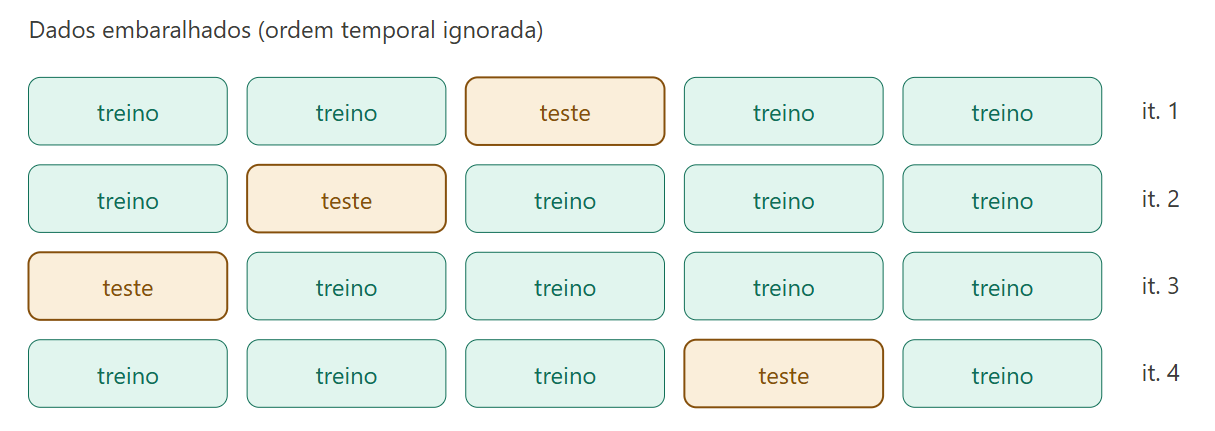
\includegraphics[width=0.85\textwidth]{figuras/referencial_teorico/kfold.png}
    \caption{Validação cruzada \textit{$K$-fold} convencional, com particionamento aleatório que desconsidera a ordem cronológica.}
    \label{fig:kfold_convencional}
    \fonte{Fonte: Elaborada pelo autor.}
\end{figure}

O pressuposto que sustenta o particionamento aleatório, contudo, é justamente o
da independência entre as observações, a mesma hipótese \textit{i.i.d.} cuja
inadequação às séries temporais foi discutida na
Subseção~\ref{subsec:fundamentos_ml}. Conforme ilustra a
Figura~\ref{fig:kfold_convencional}, o
\textit{$K$-fold} convencional permite, ao embaralhar a ordem cronológica, que observações posteriores ao instante de
previsão componham o conjunto de treinamento enquanto observações anteriores
integram o conjunto de teste, o que configuram, dessa forma, um vazamento de informação
(\textit{data leakage}) já caracterizado. Em uma série fortemente
autocorrelacionada, amostras temporalmente vizinhas são quase redundantes, de
modo que treinar com o futuro para prever o passado produz estimativas de erro
artificialmente otimistas, que não se reproduzem quando o modelo é colocado em
operação e dispõe apenas de informação pretérita \cite{hyndman2021}.


O contexto trabalhado exige, portanto, uma adaptação dos procedimentos de validação de tal forma que
toda partição respeite a ordenação temporal, dessa forma, o conjunto de avaliação deve ser
sempre posterior ao conjunto de treinamento, reproduzindo, assim, a assimetria entre
passado e futuro inerente à tarefa de previsão. Nesse sentido, a forma mais simples consiste em
uma única divisão cronológica, na qual os dados mais antigos são reservados ao
ajuste e o período mais recente, à avaliação, sendo essa estratégia adotada, por exemplo,
por \citeonline{Kappler2024}, que destinam seis anos de operação ao treinamento e
o ano subsequente à validação. Tal divisão única, no entanto, avalia o modelo
sobre um único período e fica sujeita às particularidades meteorológicas daquele
intervalo, o que limita a robustez da estimativa.

Para mitigar essa limitação preservando a causalidade temporal, emprega-se a
validação cruzada para séries temporais, em que a avaliação é repetida sobre
múltiplas divisões cronológicas sucessivas. Na variante de janela progressiva
expansiva (\textit{walk-forward} ou \textit{forward chaining}), ilustrada na
Figura~\ref{fig:walk_forward}, o horizonte de treinamento é ampliado a cada
iteração, incorporando as observações da iteração anterior, e o desempenho é
medido sempre sobre o bloco imediatamente posterior, simulando o uso real do
modelo, no qual novas observações tornam-se disponíveis com o passar do tempo. Dessa maneira, as
métricas obtidas nos sucessivos blocos de teste são então agregadas, oferecendo
uma estimativa de generalização que combina a robustez da repetição com o rigor
da separação temporal \cite{hyndman2021}. Uma forma particular dessa estratégia,
adequada a dados sazonais, é a adotada por \citeonline{Markovics2022}, que
particionam a série em blocos anuais e avaliam o modelo ajustado a um ano sobre
outro ano distinto, assegurando que treinamento e teste cubram ciclos sazonais
completos.

\begin{figure}[!h]
    \centering
    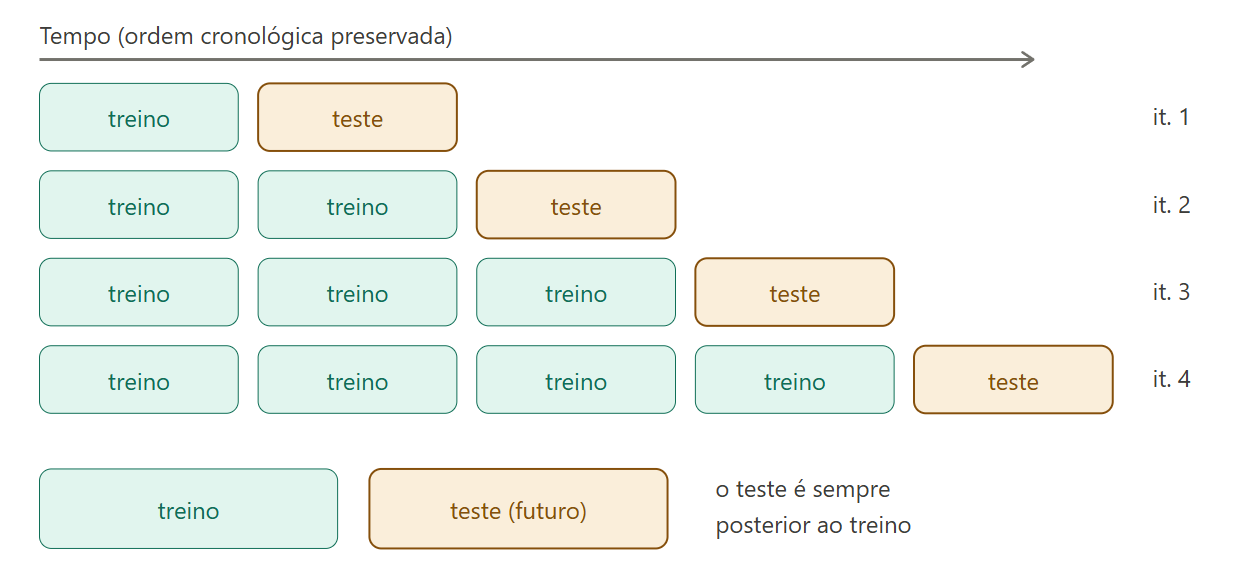
\includegraphics[width=0.85\textwidth]{figuras/referencial_teorico/walking_window.png}
    \caption{Validação cruzada em janela progressiva expansiva (\textit{walk-forward}), em que o horizonte de treinamento cresce e o teste é
    sempre o bloco posterior.}
    \label{fig:walk_forward}
    \fonte{Fonte: Elaborada pelo autor.}
\end{figure}

Uma alternativa à janela expansiva é a janela deslizante (\textit{sliding
window}), representada na Figura~\ref{fig:sliding_window}, na qual o conjunto de
treinamento mantém largura fixa e avança como um bloco rígido ao longo do tempo,
descartando as observações mais antigas à medida que incorpora as mais recentes.
A distinção entre as duas variantes não é meramente operacional, mas reflete uma
hipótese sobre a estrutura dos dados. A janela expansiva aproveita todo o
histórico disponível, reduzindo a variância das estimativas e favorecendo modelos
de maior complexidade paramétrica, que demandam mais dados para o ajuste, ao mesmo tempo, que pressupõe que os regimes passados permaneçam representativos do
futuro. Dessa forma, ao descartar deliberadamente o passado distante, a janela deslizante
torna-se mais reativa a mudanças de regime e mais fiel à condição operacional
recente, ao custo de treinar sempre com uma amostra menor. No entando, essa propriedade é
particularmente pertinente à previsão de geração fotovoltaica, na qual a
degradação gradual dos módulos e eventuais intervenções de manutenção introduzem
não-estacionariedade na série, conforme discutido na
Subseção~\ref{subsec:fundamentos_ml}, podendo tornar contraproducente o uso de dados
muito antigos no ajuste.

\begin{figure}[!h]
    \centering
    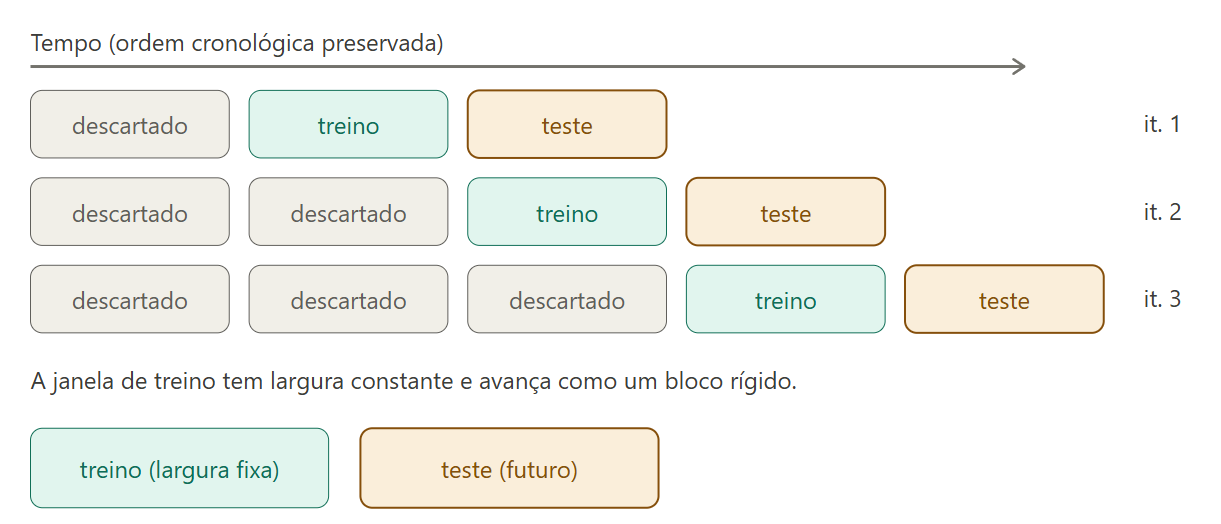
\includegraphics[width=0.85\textwidth]{figuras/referencial_teorico/sliding_window.png}
    \label{fig:sliding_window}
    \caption{Validação cruzada em janela deslizante (\textit{sliding window}), em que o conjunto de treinamento tem largura fixa e avança no tempo, descartando as observações mais antigas.}
    \fonte{Fonte: Elaborada pelo autor.}
\end{figure}

Cabe ressaltar que a validação cruzada cumpre, neste trabalho, dupla função
de estimar o desempenho final do modelo sobre dados não vistos, além de ser o instrumento
pelo qual se conduz a seleção de hiperparâmetros. Para que essa estimativa permaneça imparcial,
é necessário evitar que os dados empregados no ajuste dos hiperparâmetros
contaminem a avaliação do desempenho final, o que motiva a segregação entre
conjuntos de treinamento, e teste ou, no caso das ANN, treino, validação e teste. A definição do protocolo efetivamente adotado, incluindo a variante de janela, o número de partições e a
extensão dos blocos temporais, é apresentada no
Capítulo~\ref{cap:materiais_metodos}.